\chapter{Design and Implementation}
\label{cha:design}
\section{Toolchain}
\section{Board Configuration}
On the Hifive1, there are several important configuration options that affect general operation of the board. The most notable of these are the clock settings, as these indicate the frequency of the processor, input and output frequencies, and timer interrupts. 
\subsection{Clock settings}
% INCLUDE CLOCK USE FIGURE
The Hifive1 has 3 clock regions, a high frequency clock, a low frequency clock, and a clock used to drive the JTAG connection. The JTAG driver is constant and only used for debugging through JTAG, so is not relavent here.
\\

\begin{figure}[H]
    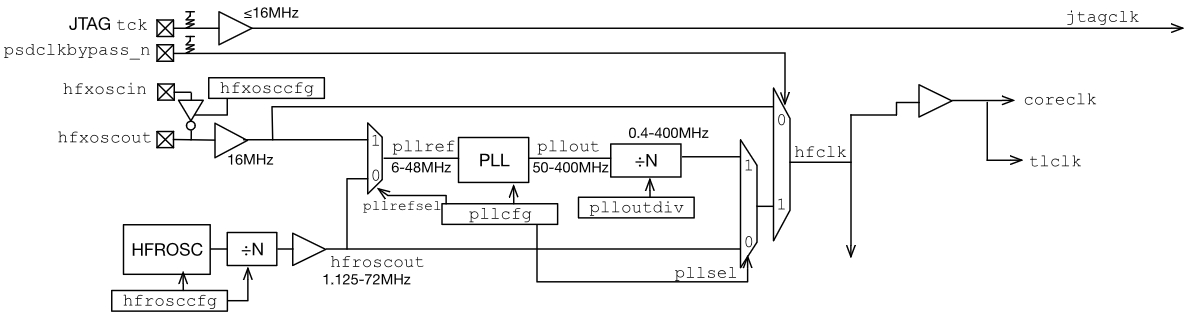
\includegraphics[width=0.9\columnwidth]{figures/hfclock.png}
    \caption[High Frequency Clock Diagram]{The high frequency clock generation scheme, specifying how the high frequency clock is driven and configured, taken from the Sifive FE310-G002 Manual CITE REFERENCE}
\end{figure}
The high frequency clock controls the processor frequency, and the baud rate of input and output is derived from it. The high frequency clock can be driven from two sources, an internally trimmable high frequency ring oscillator and an external high frequency crystal oscillator. The ring oscillator can produce frequencies ranging form ~1 MHz to 75 MHz, whereas the crytal will produce a constant frequency of 16 MHz. Both of these clock sources may be used `as is', or can be modified using a PLL and divider, giving a available range of 48 MHz to 384 MHz. 
\\
\begin{figure}[H]
    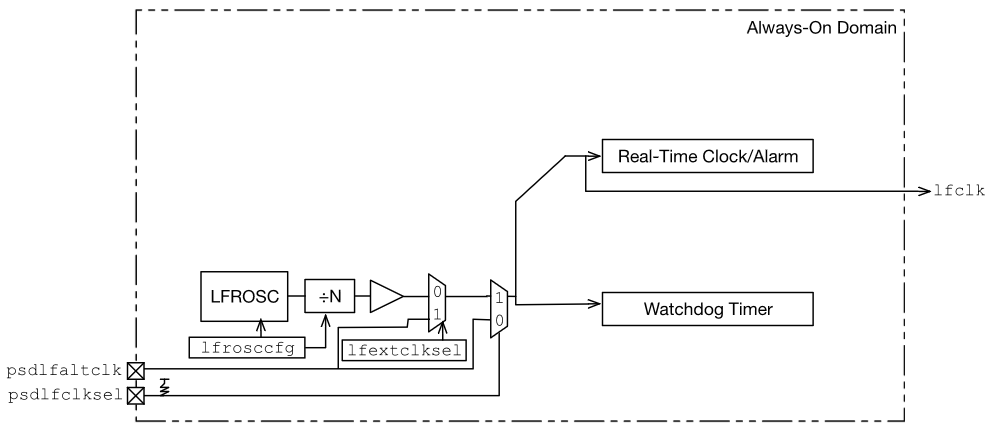
\includegraphics[width=0.9\columnwidth]{figures/lfclock.png}
    \caption[Low Frequency Clock Diagram]{The low frequency clock generation scheme, specifying how the low frequency clock is driven and configured}
\end{figure}
The low frequency clock is part of the Hifive1 `always on block' and controls the watchdog timer, which can be used to cause a reset on malfunction, and both the realtime clock and the machine timer, both of which are used to generate timed interrupts. Similar to the high frequency clock can be driven from a ring oscillator or from an external clock, which in the Hifive1 is a crystal oscillator. The low frequency ring oscillator functions at 1.5 KHz to 230 KHz using a frequency divider, and the implemented external clock runs at a contant 32.768 KHz, with no option to divide the frequency.
\\
For both clock domains, the crystal oscillator was chosen. The ring oscillator gives the option to operate at a higher frequency, which would result in a higher number of operations per second. While in a practical operating system this would be desirable, since this system is not intended for practical use, a constant frequency was more desirable as it would give more predictable results, and makes IO operations more reliable. For the low frequency clock, a high frequency would be beneficial for a real time system as the higher frequency would allow for more precise timing of interrupts and other functions, however for an interactive system this precision is not required, and so similar to the high frequency domain the constant frequency of a crystal oscillator was selected.
\section{Processes}
\subsection{Process Structure}
Due to the extremely limited amount of memory available on the Hifive1, the data required to store information on each process has to be structured carefully, else the amount of memory required to store process information would begin to limit the amount of memory available to the processes themselves. In the current implementation, 35 bytes are used to store process information.
\\
One byte each is allocated for a process id, process parent id, process status, and size of a processes text section. For process id and process parent id, only one byte is needed as the Hifive1 does not have the memory to support a large of processes, so a theorectical cap of 256 processes is acceptable. Process status can only take 4 values, so only 2 bits of the byte are used, and the text size byte stores the size as a power of 2, where a process has \(2^n\) words, where \(n\) is the value stored. While some of these values only require bits, they are stored as bytes to keep the structure word aligned. 
\\
One word each is allocated for the processes program counter, text section pointer and address space pointer. Since memory addresses are word length, these cannot be reduced.
\\
The vast majority of the process structure is used storing the 31 general purpose registers. This is required to retain the state of each process in between scheduling. The only option to reduce this would be to limit the amount of registers available to use. Only 31 must be stored as the x0 register is hardwired to zero.
\\
In other systems, information like the processes stack pointer may be stored, however standard RISC-V calling convention specifies x2 to be used as the stack pointer, so seperate storing of this infomation is not required, and allows a process to handle its address space on its own, however on process creation x2 and x3 are initialised as the stack pointer and the global pointer, where the stack pointer points to the bottom of the process address space and the global pointer at the top. This is done to reduce the overhead of processes that use the standard calling convention.
\subsection{Scheduler}
To implement an interactive system, a scheduler will be designed to allow a process run for a limited time, before halting the process, and running another ready process. The time allowed for a process to run is refered to as its quantum. Processes will be scheduled to be ran in a round robin fashion, to allow a fair runtime to each process while maintaining a low overhead. This is implemented using a circular queue, where new and halted processes are added to the end of the queue, and processes to run are taken from the start of the queue.
\section{Memory Management}
% figures, diagram of memory split into address spaces, labeled process 0 to 6 and machine memory

\section{IO}